\chapter{The Perkins Bacon Issue of 1853}

\begin{marginfigure} 
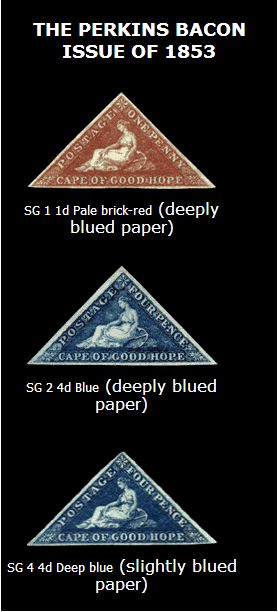
\includegraphics[width=.95\textwidth]{../cape-of-good-hope/adhesives/bacon-01.jpg}
\end{marginfigure}

The first issue of the triangular stamps of the Cape of Good Hope were engraved and printed by Messrs. Perkins, Bacon \& Co. The stamps were despatched to the Cape on the 11th May, 1853. They arrived a month later and the consignement was lodged at the Treasury Offices of the Cape. The Perkins Bacon issue was the first time that the Cape of Good Hope issued stamps.

The stamps were designed by Bell the Cape of Good Hope surveyor. The choice of the triangular shape is alleged to have been chosen so that the illiterate could distinguish the Cape of Good Hope stamps from those of other countries.

The stamps were advertized in the Cape Government Gazette of the 18th August 1853. In the same issue of the cape Government Gazette the Postamster General publishede, a long list of persons, holding retail licenses in the cape Colony, with whom arrangements were made for the sale of postage stamps.

Thus the first stamps of the Cape of Good Hope were put on Sale on 1st September 1853.

\section{The Design of the Cape Stamps}

The design of the stamps as can be seen from the above illustrations represents a female figure of Hope sitting upon an anchor, which rests upon a rock. The background consists of fine engine-turned lines. These type of background was intended to make counterfeiting difficult and was one of the selling points of Bacon's firm.

\ph[width = .45\textwidth]{../cape-of-good-hope/760_0001.jpg}{1				
PROOF OF THE BACKGROUND FOR THE G.B. 1d BLACK AND 2d BLUE - ALSO USED FOR C.G.H., N.Z., AUSTRALIAN STATES, ETC.: c.1855 Proof in blue-black on thin card (71 x 136 mm) of various designs including that used for the G.B. 1840 1d & 2d. The design was also used for various Colonial issues, so the lot includes the relevant stamps; inc. Cape of Good Hope 1855-58 4d used, Victoria 1858 6d used, South Australia 1876 2/- mint, St Vincent 1880-81 5/- mint and New Zealand 1915-22 2$\Omega$d block of four, 6d & 8d. Generally good examples. The design was also part of the NSW Diadem issue. (8 items).  zzCOMMANDzz500. Cav sep 2013}

\section{Paper Used in the Production of the Cape Stamps}

The paper used for the printing of the Cape triangular stamps was especially manufactured to the meet the particular requirements of the triangular stamps of the Cape of Good Hope. This paper was exclusively used for all the printings.

The paper is white wove varying considerably in texture. The gum is a pale brown. the gum was applied after the printing was done.

A particular aspect of this issue was the 'blueing of the paper'. This was caused entirely by the type of inks used for the printing. This effect was notable in most issues printed by Perkins, Bacon \& Co. at the time for Great Britain and its colonies.

This problem was later fixed during the printing of the Second Triangular Issue

\section{Watermark of the Cape Triangle Stamps}

The watermark used in the production of the Cape stamps was the familiar anchor in double outline. The watermark designs (technically known as 'bits') were arranged so that each stamp had one anchor standing upright, with the 'ring' underneath the apex of the triangle.

Most of the Cape triangular stamps are known with the watermark sideways. These stamps are the result of the paper being fed into the printing machine reversed, i.e. turned over so that the printing was done on the wrong side of the sheet.


Allis mentions a letter dated January 13, 1847, written by Perkins, Bacon \&Petch to Colonel Mitchell\sidenote{Lieutenant-Colonel Charles Collier Michell, (29 March 1793 Exeter - 28 March 1851 Eltham, London), later known as Charles Cornwallis Michell, was a British soldier, first surveyor-general in the Cape, road engineer, architect, artist and naturalist.}, the Surveyor General of the Colony of the Cape of Good Hope. The draft od this letter is quoted in Perkins Bacon by de Worm.

Sir,

We beg to acknowledge receipt of your Letter of the 11th Inst received last evening, asking information whether, \& at what price, `we should be willing to supply the Government of the Cape of Good Hope with stamps ready in every respect for use, \& also the black Ink used by Postmasters for Stamping 

The terms appear to have been acceptd on May 29, 1847, in a letter which is now missing, and that the order was subsequently cancelled.

Approximately five year later on 6th September 1852 an order was placed for the requisition of the first Cape of Good Hope stamps.


Gentlemen,

On the 13th of Jabuary 1847, you addressed a letter to Lt. Colonel Michell, at that time Surveyor General and Civil Engineer of this Colony, stating the terms upon which\ldots

It has also been decided to introduce a one penny for newspapers of the same shape and device but of a different colour, and with the necessary alteration of border. Of this description I am to request you to furnish an immediate first supply of fifty thousand, and a monthly remittance of five thousand, until further instructions. 

Blue has been fixed upon as the colour for the four-penny stamp and red for the one penny. 

I am further desired to transmit the enclosed device for an obliterating stamp, of which you are requested to furnish one hundred with the necessary apparatus of dabbers \&c for defacing stamps and a supply of 250 lbs of obliterating ink.

The label sheets hereby directed to be forwarded you will, as a matter of course, have gummed in every way ready for immediate service.

In conclusion I have to add, that payment of the expense for this order will be made by the Agent General for Crown Colonies upon the completion of the work, in terms of the conditions specified.

I have the honor to be, Gentlemen

Your most obedt Servant

J Winkley

Actg Secy to Government

The letter, besides its historical importance to the first postage stamps of the Cape of Good Hope, it also gives us a glimpse of the items of post used montthly, especially the newspapers and the number of the first triangular obliterators. It is interesting to note that the amount of letters at the time was about twice that of newpapers (and the same was true when the second order  was placed in October 1853).

On November 4, Perkin Bacon's tender was accepted, with the only provision that 'fifty pounds of the Ink only to be sent', and forwarded by Edward Barnard to Perkins, Bacon on official instructions.

The Engraving Records show that the drawing was ready by November 10, but the dies were not completed until February 16, 1853.


\section{Second Order}

The quantity of the monthly supply were revised in October 1853:

{\ttfamily
5, Cannon Row, Westminster

13th Octr. 1853.

Gentlemen

I have to request that you will provide for the service of the Government of the Cape of Good Hope 200,000 fourpenny Stamps (Blue) and 100,000 stamps (Red) in place of the monthly supply of the postage stamps originally ordered.

The Packages are to be addressed,
\begin{verbatim}
                 The Officer
                     Administering the Government
                         Cape of Good Hope
\end{verbatim}
and forwarded to teh order of Mr. Winkley, Shipping Agent, 23, Birchin Lane, Cornhill; transmitting at the same time, to this office, three copies of the Invoice, which must state the number of Packages.
}




















                                                 